\documentclass[letterpaper, 10pt, conference]{ieeeconf}      % Use this line for a4
                                                          % paper

\IEEEoverridecommandlockouts                              % This command is only
                                                          % needed if you want to
                                                          % use the \thanks command
\overrideIEEEmargins
% See the \addtolength command later in the file to balance the column lengths
% on the last page of the document

%\setlength{\topmargin}{0.46in}

% The following packages can be found on http:\\www.ctan.org
\usepackage{graphics} % for pdf, bitmapped graphics files
\usepackage{epsfig} % for postscript graphics files
%\usepackage{mathptmx} % assumes new font selection scheme installed
\usepackage{times} % assumes new font selection scheme installed
\usepackage{amsmath} % assumes amsmath package installed
%\usepackage{amssymb}  % assumes amsmath package installed
\usepackage{wasysym}
\usepackage{color}
\usepackage{algorithmic}

%\usepackage[dvips, bookmarks=false, colorlinks=true, pdftitle={Hak-TSMC2011}]{hyperref}
\newcommand{\mbf}[1]{{\mathbf{#1}}}
\newcommand{\dpartial}[2]{\frac{\partial{#1}}{\partial{#2}}}
\DeclareMathOperator*{\argmin}{arg\,min\,} 



\author {Sovannara Hak, Nicolas Mansard, Olivier Stasse, Jean-Paul Laumond}
\title{Humanoid Robot Task Recognition from Movement Analysis - Abstract}
\begin{document}
\maketitle

We present a method to perform tasks identification on a
humanoid robot. The approach is to formulate
the problem of tasks identification as a problem of
selection of controllers in a finite set~(Fig.~\ref{fig:observation}). 
\begin{figure}[t]
\begin{center}
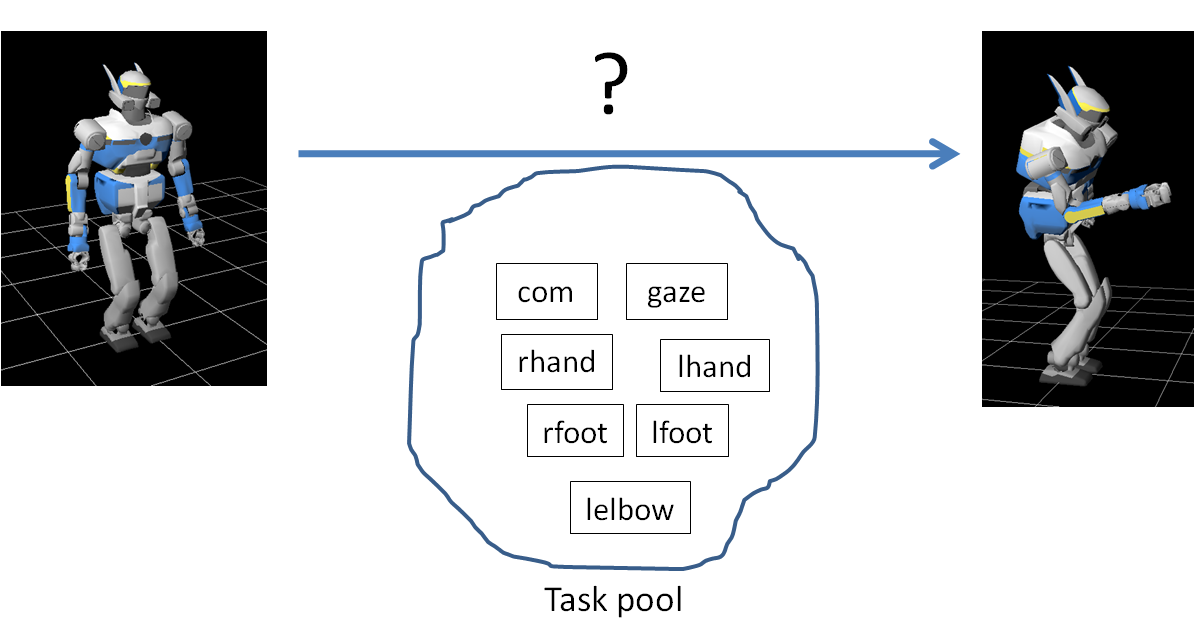
\includegraphics[width=0.8\linewidth]{img/observation.ps}
\end{center}
\caption{Selection of the controllers that would generate the observed movement.}
\label{fig:observation}
\end{figure}

The selection of the relevant controllers is based on a movement analysis
that performs a reverse engineering of the humanoid motion.
The selected controllers can be used as a description of the motion, or as
a basis to replicate a similar motion on another robot~(Fig.~\ref{fig:identification}).
\begin{figure}[t]
\begin{center}
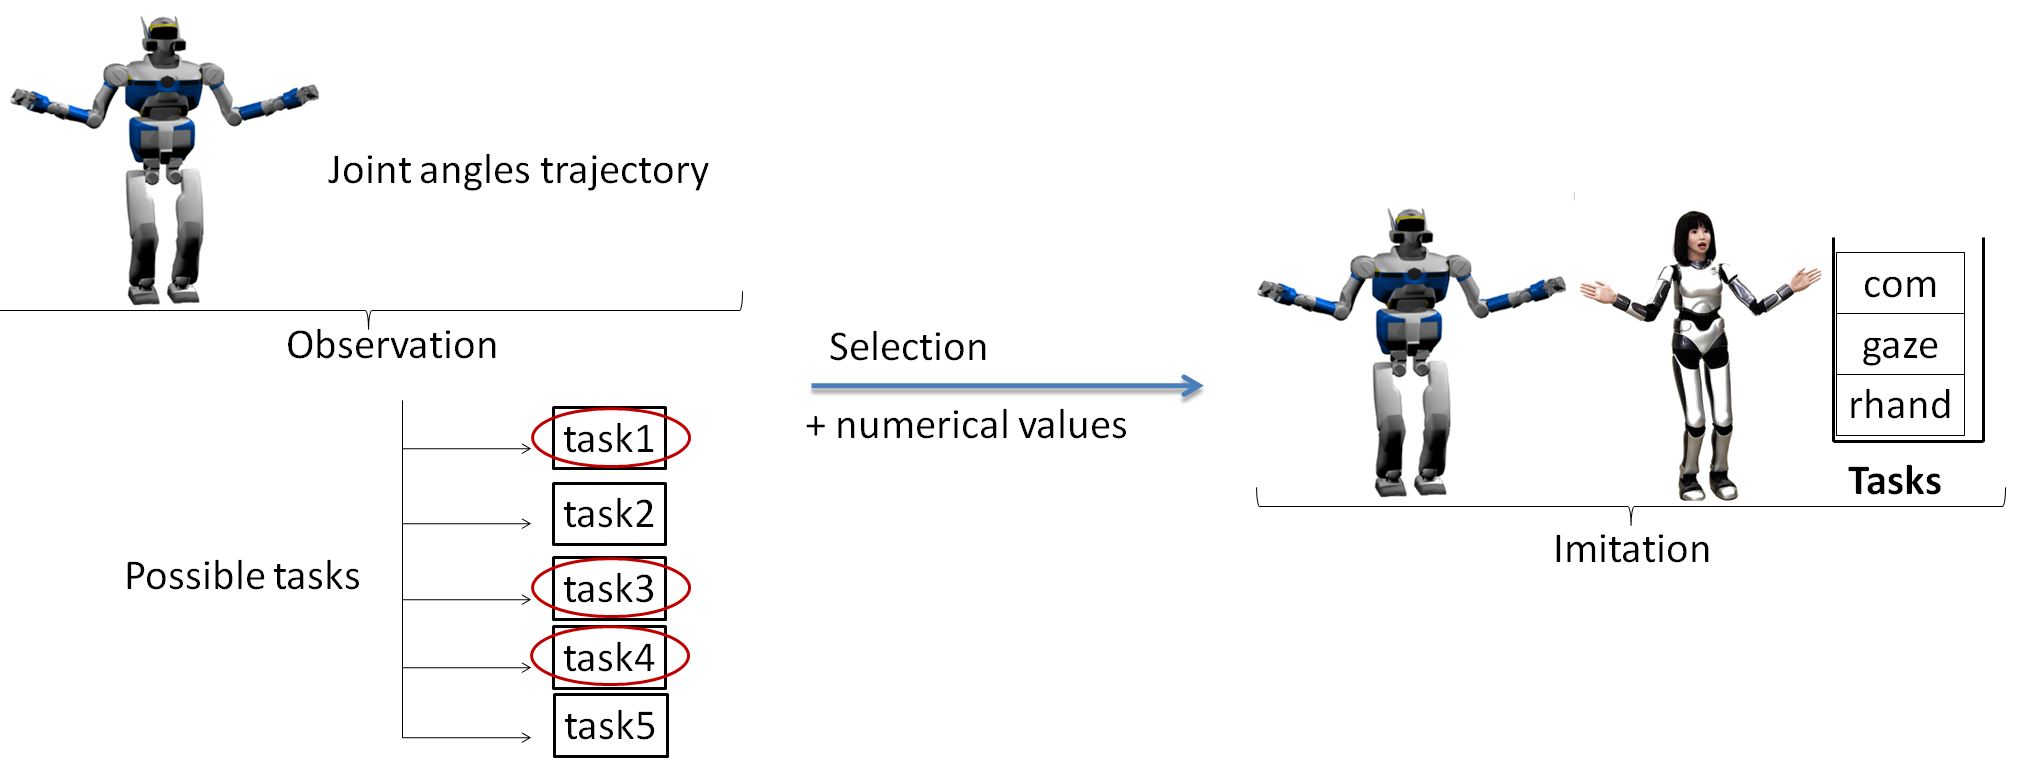
\includegraphics[width=\linewidth]{img/identification.ps}
\end{center}
\caption{A reverse engineering technique is performed to reconstruc the stack of tasks
used in the demonstration.}
\label{fig:identification}
\end{figure}

The analysis of the movements is based on the task-function approach and is
applied in the context of humanoid robot motions.  A pool of tasks is defined
in order to cover the range of possible motion of the robot and the
movement to analyze is projected in each candidate task of that pool. 
The reduced trajectory is then compared with the characteristic task trajectory
using a numerical optimization process and its residue is used as a 
decision criterion~(Fig.~\ref{fig:projection}).
\begin{figure}[t]
\begin{center}
\includegraphics[width=0.9\linewidth]{img/projection.ps}
\end{center}
\caption{Projection of the motion in the tasks space and comparison with
theorical trajectories to select the relevant tasks. Here the gaze task is relevant,
and the left hand task is not.}
\label{fig:projection}
\end{figure}

In order to identify a set of tasks involved in a movement, an iterative
process is used. The initial movement is projected into the null space of the
selected task candidate. This projection will remove the motion due to the
selected task from the original movement. As a consequence,
the analysis of the projected movement will not be influenced by
the selected task. An example of projected movement is showed in~(Fig.~\ref{fig:nullspace})
where the first row shows the original movement, and the last row shows the
remaining movement after successive projection into the nullspace of the tasks
: right hand, center of mass, gaze, feet relative position, left hand.
\begin{figure}[t]
\begin{center}
\includegraphics[width=0.9\linewidth]{img/nullspaceProjection.ps}
\end{center}
\caption{Projecting a motion in the nullspace of a task, remove the motion
	due to that task. }
\label{fig:nullspace}
\end{figure}

This process is iterated until the result of a projection leads to a null motion,
which means that all the tasks involved in the original motion
have been deleted, and therefore selected~(Fig.~\ref{fig:algorithm}).
\begin{figure}[t]
\begin{center}
%\includegraphics[height=0.9\linewidth, angle = -90]{img/PqdotNorms.ps}
\resizebox{.48\textwidth}{!} {
      \input{img/PqdotNorms.pstex_t}
    }
\end{center}
\caption{Successive projection into the nullspace of tasks until the norm of the
	velocity of the robot joint angle becomes null. $P_i$ is the nullspace projection
	operator for the task $i$.}
\label{fig:algorithm}
\end{figure}

Removing the motion due to a task allow to disambiguate very similar-looking motions
because it will remove all the secondary motions that contribute to the main task.
For example, for a reaching task, the humanoid robot may bend his chest to
reach the desired position. This chest motion will be removed when the motion
will be projected into the nullspace of the hand task. On the other hand,
if the motion of the chest is defined as a proper task, the projection into the
nullspace of the hand task, will not remove all the motion in the chest.

The approach is applied to recognize the tasks performed by a HRP-2 robot in simulation
and on the real robot (using a motion capture system to acquire motion data), in order to
disambiguate very similar-looking motions. To illustrate the performance
of the method, three disambiguations are detailed
\footnote{Videos are available {http://homepages.laas.fr/shak/videos/}} :
\begin{itemize}
\item a motion involving a task with the right hand and another with both hands~(Fig.~\ref{fig:spotDiff1})
\item a 3D position task for a grab motion, and another involving 6D position 
task for a screwing motion~(Fig.~\ref{fig:spotDiff2})
\item a \emph{gaze} motion, and a \emph{screw} motion~(Fig.~\ref{fig:spotDiff3})
\end{itemize}

\begin{figure}[t]
\begin{center}
\includegraphics[width=0.7\linewidth]{img/spotDiff1.ps}
\end{center}
\caption{Top: the final posture of the robot with only the right hand task; Bottom:
the final posture with a left and right hand tasks. The colored ball represent the desired positions.}
\label{fig:spotDiff1}
\end{figure}

\begin{figure}[t]
\begin{center}
\includegraphics[width=0.7\linewidth]{img/spotDiff2bis.ps}
\end{center}
\caption{Left: The final position of the grab motion; Right: The final position of the screwing motion.}
\label{fig:spotDiff2}
\vspace{-3pt}
\end{figure}

\begin{figure}[t]
\begin{center}
\includegraphics[width=0.7\linewidth]{img/spotDiff3.ps}
\end{center}
\caption{Left: The final position of the gaze motion; Right: The final position of the grab motion.}
\label{fig:spotDiff3}
\end{figure}

\end{document}







